\begin{frame}
  \begin{PointSix}{Houskeeping}
    \begin{itemize}
      \item \alert{Geophysics at seminar 20.05.2022}
      \item \alert{Questions regarding exercises}
    \end{itemize}
  \end{PointSix}
\end{frame}

\begin{frame}
  \begin{PointSix}{Learning Goals}
    \begin{itemize}
      \item \alert{Understand the principle of the resistivity method.}
      \item \alert{Understand basic electrostatic principles.}
      \item \alert{Understand principles of vertical sounding.}
    \end{itemize}
  \end{PointSix}
\end{frame}

\begin{frame}
  \begin{PointSix}{Resistivity Method Principles}
      \small
      Characterize the sub-surface in it's ability to conduct electrical currents. A material that has a high electrical resistivity will conduct electrical currents poorly and vice versa.
  \end{PointSix}
\end{frame}

\begin{frame}
  \begin{PointSix}{Principle of the resistivity method}
   % RESISTOR with battery and arrow

    \begin{tikzpicture}
      
      \newcommand\EMF{\mathcal{E}};
      \colorlet{Icol}{blue!50!black}
      \colorlet{Ccol}{orange!90!black}
      \colorlet{Rcol}{Karminrot}
      \colorlet{loopcol}{red!90!black!25}
      \colorlet{pluscol}{red!60!black}
      \colorlet{minuscol}{blue!60!black}
      \tikzstyle{EMF}=[battery1,l=$\EMF$];
      \tikzstyle{internal R}=[R,color=Rcol,Rcol,l=$r$,/tikz/circuitikz/bipoles/length=30pt];
      \tikzstyle{loop}=[->,red!90!black!25];
      \tikzstyle{loop label}=[loopcol,fill=white,scale=0.8,inner sep=1];
      \tikzstyle{thick R}=[R,color=Rcol,thick,Rcol,l=$R$];
      
      \begin{scope}[rotate=-90,transform shape]
        \fill[pattern = crosshatch dots,pattern color = brown!80!red] (0.5,-0.5) rectangle ++(6,9);
        \node[rotate=90] at (0.25,1.5) {Surface};
        \draw (0,8) to [short,*-] (4,8) to[R,color=Rcol,thick,l={{{{\rotatebox[origin=c]{90}{$R$}}}}}] (4,0) to [short,-*] (0,0);
        \node[rotate=90,above] at (0,8) {$+$};
        \node[rotate=90,above] at (0,0) {$-$};
        \node[rotate=90] at (0,4) {$\Delta V$};
          %  \draw[->,red] (0.5, 2.15) --++ (1.2,0) node[midway,above=1] {current $I$};
          %  \draw[->,red] (0.5,-0.15) --++ (1.2,0) node[midway,below=1] {electron flow};
          \end{scope}
    \end{tikzpicture}
  \end{PointSix}
\end{frame}

\begin{frame}
     \begin{PointSix}{Resistivity vs. Resistance}
      \begin{center}
        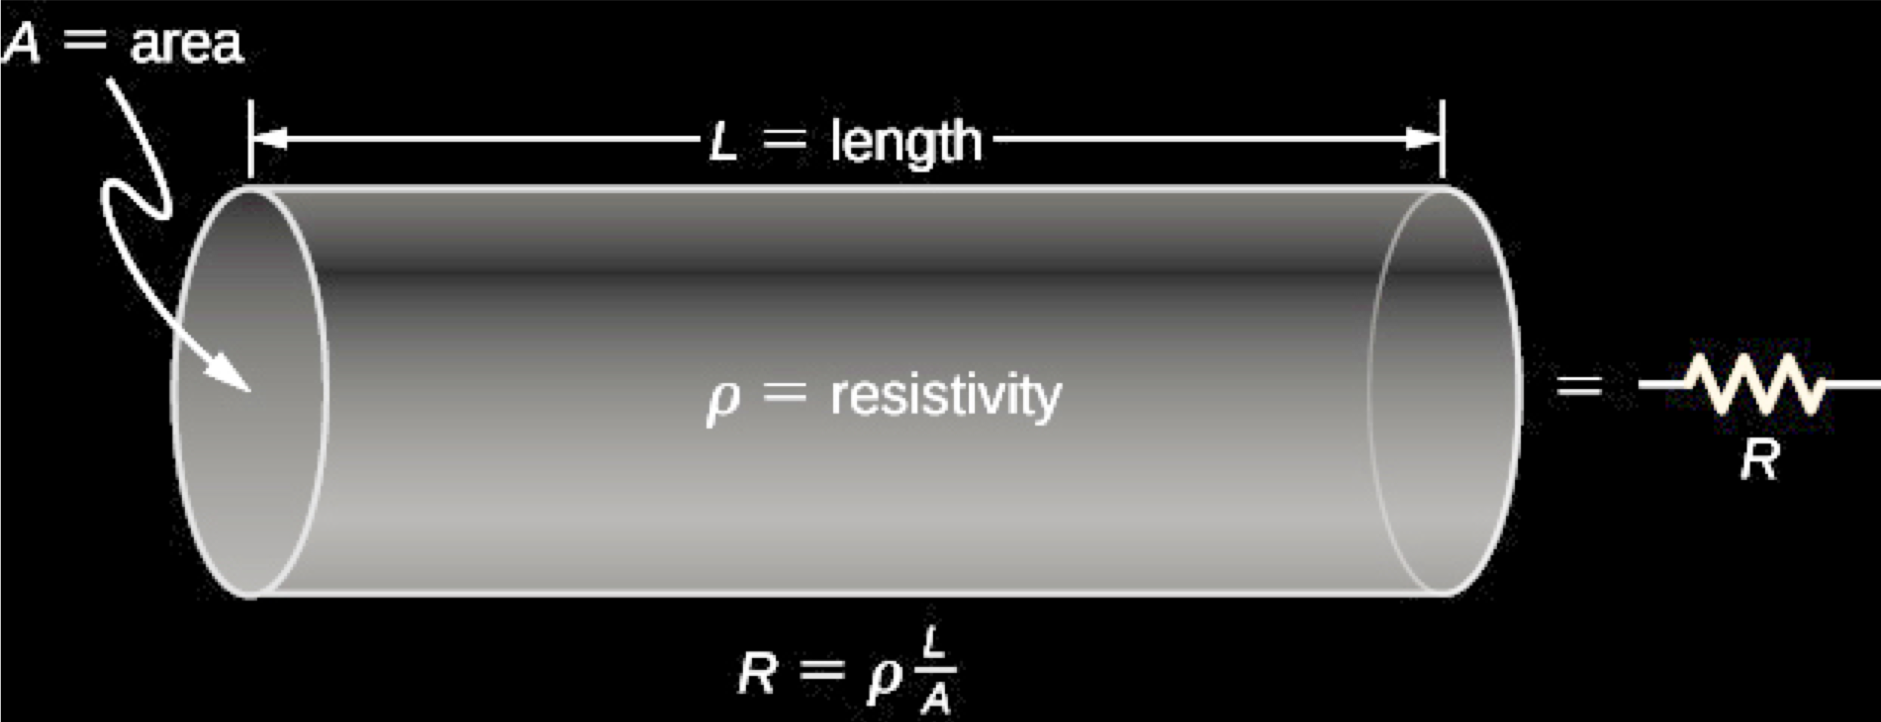
\includegraphics[width=0.90\linewidth]{Figures/Resistivity/ResistanceResistivity.png}
      \end{center}
      \small
      \begin{itemize}
        \item Resistivity (spez. elektr. Widerstand) is a material property
        \item Resistance (elektr. Widerstand) includes material and geometry of the resistor
      \end{itemize}
      \end{PointSix}
\end{frame}

\begin{frame}
  \begin{PointSix}{Resistivity vs. Resistance}
   \begin{center}
     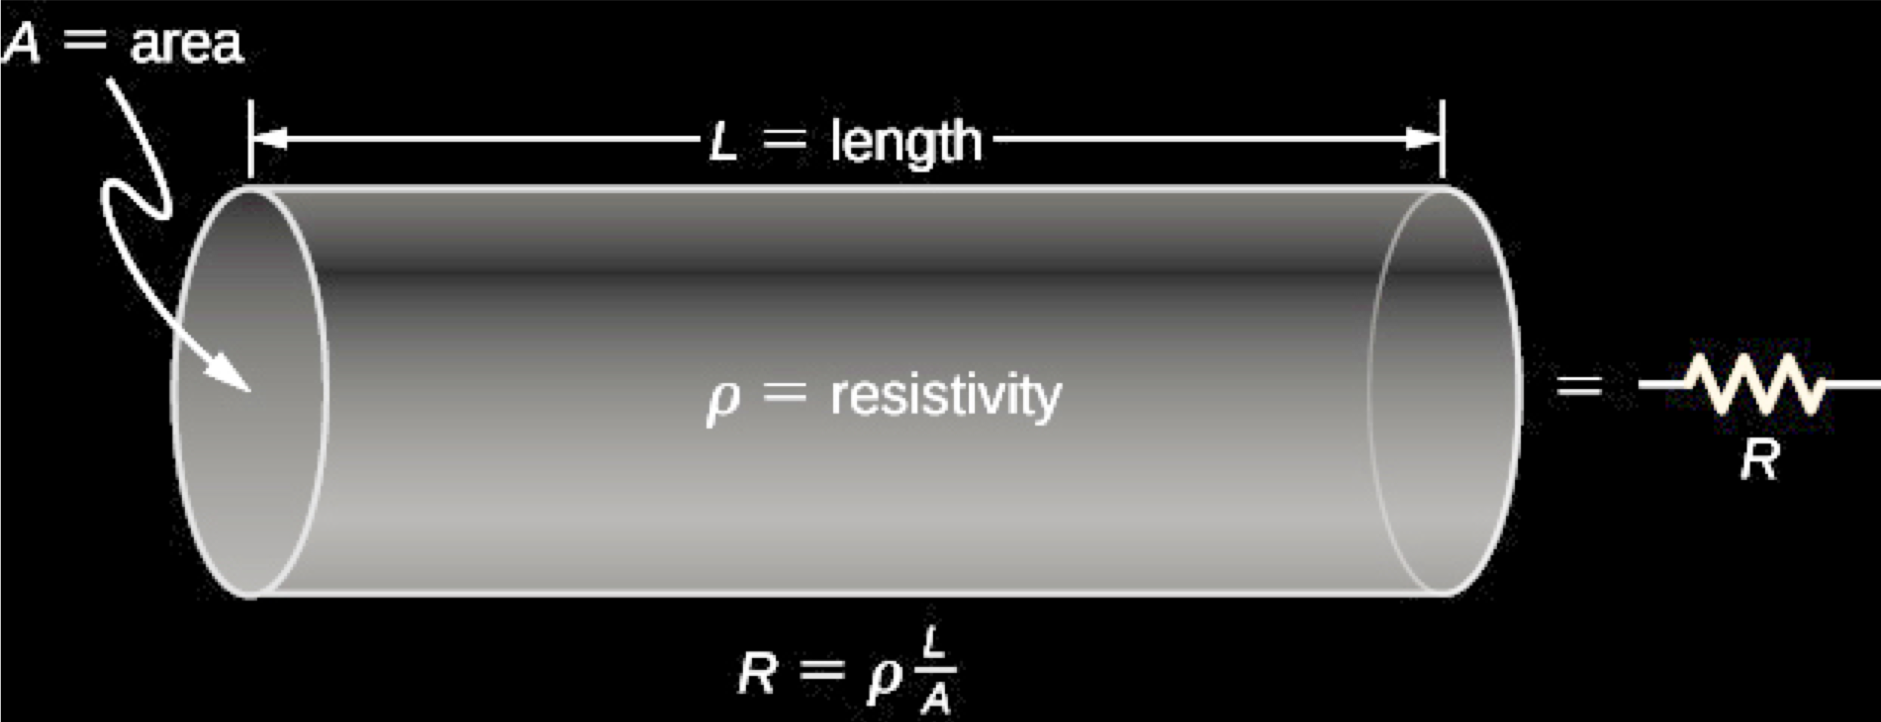
\includegraphics[width=0.90\linewidth]{Figures/Resistivity/ResistanceResistivity.png}
   \end{center}
   \small
   \begin{itemize}
     \item Resistance [Ohm, $\Omega$]
     \item Resistivity [$\Omega m$]
   \end{itemize}
   \end{PointSix}
\end{frame}

\begin{frame}
  \begin{PointSix}{Resistivity ($\rho$) vs. Conductivity ($\sigma$)}
   \begin{center}
     $$
      \rho = \frac{1}{\sigma}
     $$
   \end{center}
   \small
   \begin{itemize}
     \item Resistivity [$\Omega m$]
     \item Conductivity [$(\Omega m)^{-1}$, i.e. Siemens]
   \end{itemize}
   \end{PointSix}
\end{frame}

\begin{frame}
  \begin{PointSix}{Ionic vs. metallic conduction}
    \begin{center}
      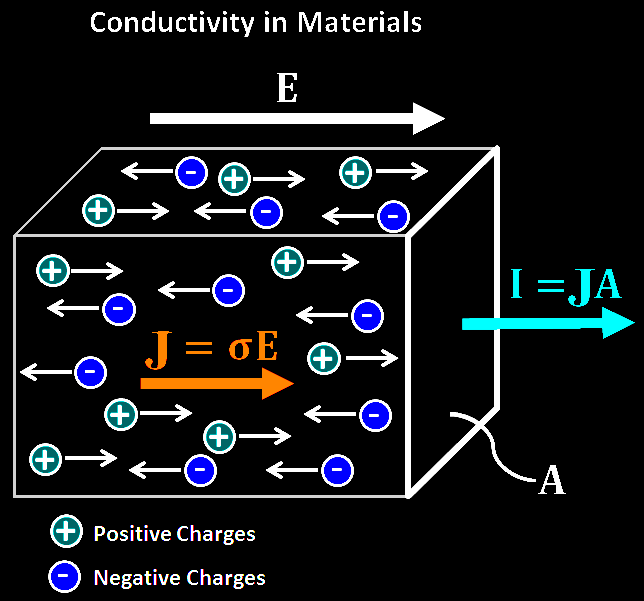
\includegraphics[width=0.80\linewidth]{Figures/Resistivity/conductivity_physics_diagram_RGeoSciXYZ.png}
      \tiny[GeoSci XYZ]
    \end{center}
   
      
  \end{PointSix}
\end{frame}

\begin{frame}
  \begin{PointSix}{Ionic vs. metallic}
    \begin{center}
      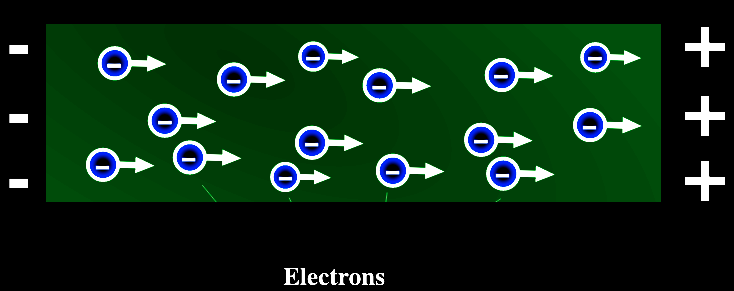
\includegraphics[width=0.90\linewidth]{Figures/Resistivity/MetallicCondution.png}
     % \tiny[GeoSci XYZ]
    \end{center}
    \small
    \begin{itemize}
      \item \alert{Metallic conduction} uses declocalized electrons in the conduction band of metalls
      \item \alert{Ionic conduction} uses charged Ions in electrolyt 
    \end{itemize}
    \end{PointSix}
\end{frame}
\begin{frame}
  \begin{PointSix}{Ionic conduction in porous sediments}
    \begin{center}
      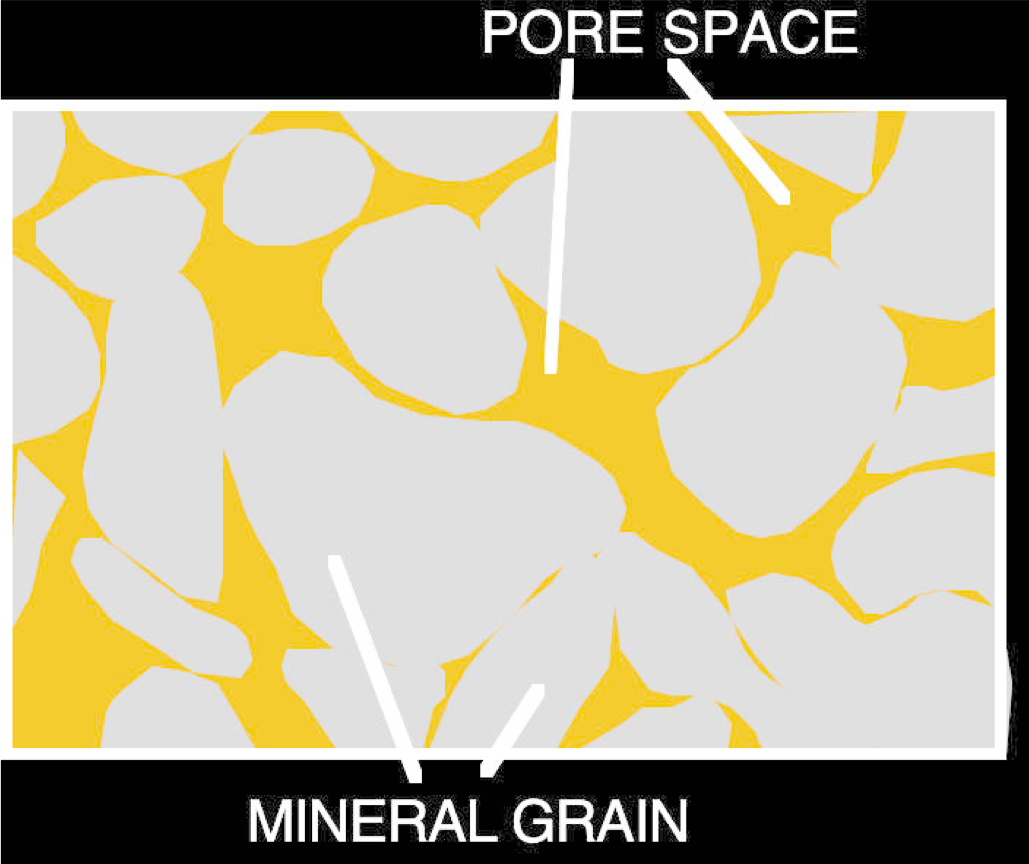
\includegraphics[width=0.90\linewidth]{Figures/Resistivity/ProusMedia.png}
     % \tiny[GeoSci XYZ]
    \end{center}
    \end{PointSix}
\end{frame}

\begin{frame}
  \begin{PointSix}{Ionic conduction in porous sediments}
    \small
    \begin{itemize}
      \item Increases with increasing pore space ($\phi$)
      \item Increases with increasing water saturation
      \item Increases with decreasing water resistivity ($\rho$)
    \end{itemize}
    \normalsize
    \onslide<2>{
      \begin{equation}
        \rho_t = a\rho_w\phi^{-m}s_w^{-n}
      \end{equation}
      \begin{center}
       \small (Archie's Law)
      \end{center}
      
      }
    \end{PointSix}
\end{frame}

\begin{frame}
 % \begin{PointSix}{Huge spread in material properties}
   % RESISTOR with battery and arrow
   \begin{center}
    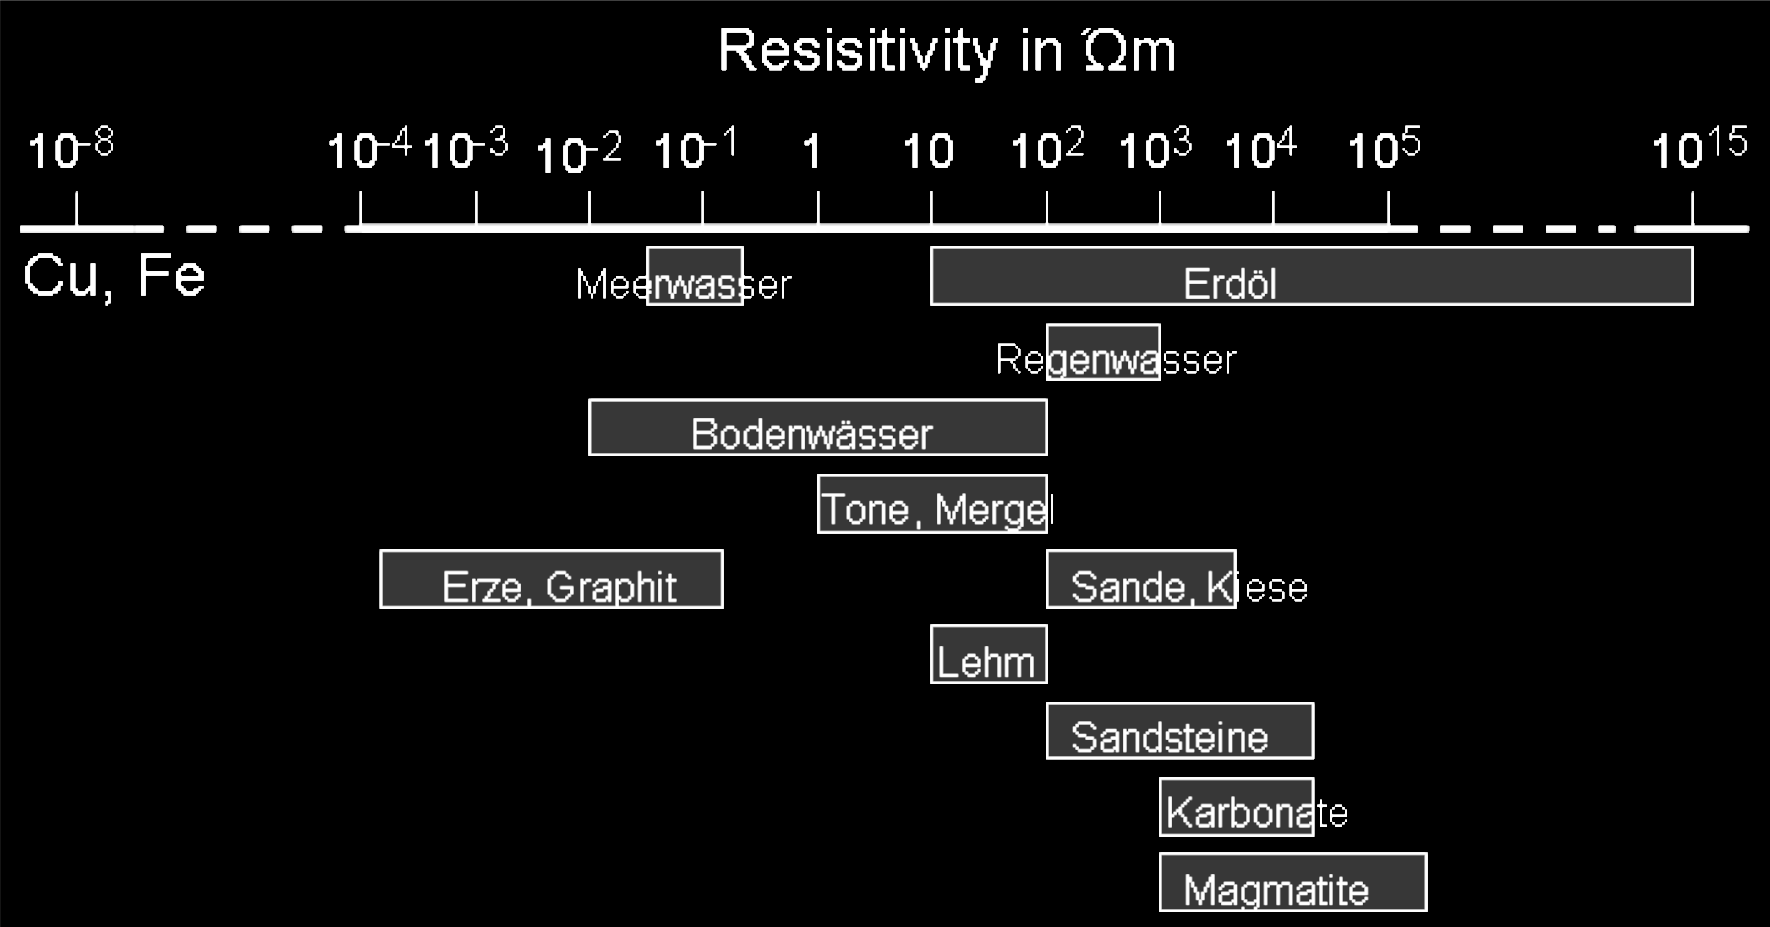
\includegraphics[width=0.8\linewidth]{Figures/Resistivity/ResistivityMaterials.png}
    
  \end{center}
  %\end{PointSix}
\end{frame}

\begin{frame}{Current flow through the sub-surface}
  \begin{PointSix}{Current flow through the sub-surface}
    \small
    Consider a homogeneous conducting halfspace, with constant resistivity $\rho$, under an insulating medium. Let there be a point electrode at the surface
injecting a steady current I. The current flows to a distributed sink at infinity. Find the electrostatic potential, the electric field, and consequently the pattern of current flow in the sub-surface.
  \\
  \vspace{1 cm}
  \tiny  [cf. Telford Chapter 8, online resources resistivity 1 and resistivity 2.]
  \end{PointSix}
\end{frame}

\begin{frame}{Current flow through the sub-surface}
  \begin{PointSix}{Primary parameter of the resistivity method}
   % RESISTOR with battery and arrow
   \begin{center}
    \begin{tikzpicture}
      \coordinate (A) at (8,0);
      \coordinate (B) at (4,-0.5);
      \coordinate (C) at (5,-3.5);
      \coordinate (D) at (6,-3.5);
      \draw [thick] (0,0.0) -- (8,0.0);
      % drawing the node with shape=rectangle and anchor=center
      %\node [draw, Karminrot, thick, shape=rectangle, minimum width=0.25cm, minimum height=0.25cm, anchor=center] at (B) {};
      \draw [->, line width = 1mm] (4,0.5) -- (B) node[xshift=1.0cm,yshift=1.0cm,midway,left] {current $\vec{I}$};;
  
      \node[yshift=0.3cm] at (A) {\small Surface};
  
    \end{tikzpicture}
    % $$
    %   \boxed{\vec{j} = \sigma \vec{E}}
    % $$
    % \small
    % $\vec{E}$ is the electrical field ($V m^{-1}$ )\\
    % $\vec{j}$ is the current density ($A m^{-2}$) \\
    % \vspace{1cm}
    % \alert{Currents flow parallel to the electrical field.}
  \end{center}
  \end{PointSix}
\end{frame}

\begin{frame}
  \begin{PointSix}{Current flow through the sub-surface}
   % RESISTOR with battery and arrow
   \begin{center}
    \begin{tikzpicture}
      \coordinate (A) at (8,0);
      \coordinate (B) at (4,-0.5);
      \coordinate (C) at (5,-3.5);
      \coordinate (D) at (6,-3.5);
      \draw [thick] (0,0.0) -- (8,0.0);
      % drawing the node with shape=rectangle and anchor=center
      %\node [draw, Karminrot, thick, shape=rectangle, minimum width=0.25cm, minimum height=0.25cm, anchor=center] at (B) {};
      \draw [->, line width = 1mm] (4,0.5) -- (B) node[xshift=1.0cm,yshift=1.0cm,midway,left] {current $\vec{I}$};;
  
      \node[yshift=0.3cm] at (A) {\small Surface};
  
    \end{tikzpicture}
    $$
      \boxed{\vec{j} = \sigma \vec{E}}
    $$
    \small
    $\vec{E}$ is the electrical field ($V m^{-1}$ )\\
    $\vec{j}$ is the current density ($A m^{-2}$) \\
    \vspace{1cm}
    \alert{Currents flow parallel to the electrical field.}
  \end{center}
  \end{PointSix}
\end{frame}

\begin{frame}
  \begin{PointSix}{Current flow through the sub-surface}
   % RESISTOR with battery and arrow
   \begin{center}
    \begin{tikzpicture}
      \coordinate (A) at (8,0);
      \coordinate (B) at (4,-0.5);
      \coordinate (C) at (5,-3.5);
      \coordinate (D) at (6,-3.5);
      \draw [thick] (0,0.0) -- (8,0.0);
      % drawing the node with shape=rectangle and anchor=center
      %\node [draw, Karminrot, thick, shape=rectangle, minimum width=0.25cm, minimum height=0.25cm, anchor=center] at (B) {};
      \draw [->, line width = 1mm] (4,0.5) -- (B) node[xshift=1.0cm,yshift=1.0cm,midway,left] {current $\vec{I}$};;
  
      \node[yshift=0.3cm] at (A) {\small Surface};
  
    \end{tikzpicture}
    $$
      \boxed{\vec{j} = \sigma \vec{E}}
    $$
    \small
    $\vec{E}$ is the electrical field ($V m^{-1}$ )\\
    $\vec{j}$ is the current density ($A m^{-2}$) \\
    \vspace{1cm}
    \alert{This is the vector version of Ohm's law (U = RI)}
  \end{center}
  \end{PointSix}
\end{frame}


\begin{frame}
  \begin{PointSix}{Current flow through the sub-surface}
   % RESISTOR with battery and arrow
   \begin{center}
    \begin{tikzpicture}
      \coordinate (A) at (8,0);
      \coordinate (B) at (4,-0.5);
      \coordinate (C) at (5,-3.5);
      \coordinate (D) at (6,-3.5);
      \draw [thick] (0,0.0) -- (8,0.0);
      % drawing the node with shape=rectangle and anchor=center
      %\node [draw, Karminrot, thick, shape=rectangle, minimum width=0.25cm, minimum height=0.25cm, anchor=center] at (B) {};
      \draw [->, line width = 1mm] (4,0.5) -- (B) node[xshift=1.0cm,yshift=1.0cm,midway,left] {current $\vec{I}$};;
  
      \node[yshift=0.3cm] at (A) {\small Surface};
  
    \end{tikzpicture}
    $$
      \vec{j} = \sigma \vec{E} = \sigma \nabla V
    $$
    \small
    %\vspace{1cm}
    \alert{The electrical field is perpendicular to the electric potential (Volts).}
  \end{center}
  \end{PointSix}
\end{frame}

\begin{frame}
  \begin{PointSix}{Current flow through the sub-surface}
   % RESISTOR with battery and arrow
   \begin{center}
    \begin{tikzpicture}
      \coordinate (A) at (8,0);
      \coordinate (B) at (4,-0.5);
      \coordinate (C) at (5,-3.5);
      \coordinate (D) at (6,-3.5);
      \draw [thick] (0,0.0) -- (8,0.0);
      % drawing the node with shape=rectangle and anchor=center
      %\node [draw, Karminrot, thick, shape=rectangle, minimum width=0.25cm, minimum height=0.25cm, anchor=center] at (B) {};
      \draw [->, line width = 1mm] (4,0.5) -- (B) node[xshift=1.0cm,yshift=1.0cm,midway,left] {current $\vec{I}$};;
  
      \node[yshift=0.3cm] at (A) {\small Surface};
  
    \end{tikzpicture}
    $$
      \nabla\cdot\vec{j} = 0
    $$
    \small
    %\vspace{1cm}
    \alert{In the half space there are no sources and sinks for the current density. Understand this from what we learned about the magnetic dipole field which is also divergence free.}
  \end{center}
  \end{PointSix}
\end{frame}



\begin{frame}
  \begin{PointSix}{Current flow through the sub-surface}
   % RESISTOR with battery and arrow
   \begin{center}
    \begin{tikzpicture}
      \coordinate (A) at (8,0);
      \coordinate (B) at (4,-0.5);
      \coordinate (C) at (5,-3.5);
      \coordinate (D) at (6,-3.5);
      \draw [thick] (0,0.0) -- (8,0.0);
      % drawing the node with shape=rectangle and anchor=center
      %\node [draw, Karminrot, thick, shape=rectangle, minimum width=0.25cm, minimum height=0.25cm, anchor=center] at (B) {};
      \draw [->, line width = 1mm] (4,0.5) -- (B) node[xshift=1.0cm,yshift=1.0cm,midway,left] {current $\vec{I}$};;
  
      \node[yshift=0.3cm] at (A) {\small Surface};
  
    \end{tikzpicture}
    $$
    \nabla \cdot \vec{j} = \sigma \nabla \cdot \vec{E} = \sigma \nabla^2 V =0
    $$
    \small
    %\vspace{1cm}
    \alert{This is the Laplace equation.}
  \end{center}
  \end{PointSix}
\end{frame}

\begin{frame}
  \begin{PointSix}{Current flow through the sub-surface}
   % RESISTOR with battery and arrow
   \begin{center}
    \begin{tikzpicture}
      \coordinate (A) at (8,0);
      \coordinate (B) at (4,-0.5);
      \coordinate (C) at (5,-3.5);
      \coordinate (D) at (6,-3.5);
      \draw [thick] (0,0.0) -- (8,0.0);
      % drawing the node with shape=rectangle and anchor=center
      %\node [draw, Karminrot, thick, shape=rectangle, minimum width=0.25cm, minimum height=0.25cm, anchor=center] at (B) {};
      \draw [->, line width = 1mm] (4,0.5) -- (B) node[xshift=1.0cm,yshift=1.0cm,midway,left] {current $\vec{I}$};;
  
      \node[yshift=0.3cm] at (A) {\small Surface};
  
    \end{tikzpicture}
    \begin{eqnarray*}
    &\nabla \cdot \vec{j} = \sigma \nabla \cdot \vec{E} = \sigma \nabla^2 V =0 \\
    &\rightarrow V = \frac{A}{r}
    \end{eqnarray*}
    \small
    %\vspace{1cm}
    (Exercises)\\
    \alert{The current flows radially outwards.}
  \end{center}
  \end{PointSix}
\end{frame}

\begin{frame}
  \begin{PointSix}{Current flow through the sub-surface}
   % RESISTOR with battery and arrow
   \begin{center}
    \begin{tikzpicture}
      \coordinate (A) at (8,0);
      \coordinate (B) at (4,-0.5);
      \coordinate (C) at (5,-3.5);
      \coordinate (D) at (6,-3.5);
      \draw [thick] (0,0.0) -- (8,0.0);
      % drawing the node with shape=rectangle and anchor=center
      %\node [draw, Karminrot, thick, shape=rectangle, minimum width=0.25cm, minimum height=0.25cm, anchor=center] at (B) {};
      \draw [->, line width = 1mm] (4,0.5) -- (B) node[xshift=1.0cm,yshift=1.0cm,midway,left] {current $\vec{I}$};;
  
      \node[yshift=0.3cm] at (A) {\small Surface};
  
    \end{tikzpicture}
    \begin{eqnarray*}
    I &=& 2\pi r^2 j \\   
      &=& -2\pi r^2 \sigma \nabla \phi \\
      &=& 2\pi \sigma A
    \end{eqnarray*}
    $$
    A = -\frac{I\rho}{4\pi}
    $$
    \small
  \end{center}
  \end{PointSix}
\end{frame}

\begin{frame}
  \begin{PointSix}{Current flow through the sub-surface}
   % RESISTOR with battery and arrow
   \begin{center}
    \begin{tikzpicture}
      \coordinate (A) at (8,0);
      \coordinate (B) at (4,-0.5);
      \coordinate (C) at (5,-3.5);
      \coordinate (D) at (6,-3.5);
      \draw [thick] (0,0.0) -- (8,0.0);
      % drawing the node with shape=rectangle and anchor=center
      %\node [draw, Karminrot, thick, shape=rectangle, minimum width=0.25cm, minimum height=0.25cm, anchor=center] at (B) {};
      \draw [->, line width = 1mm] (4,0.5) -- (B) node[xshift=1.0cm,yshift=1.0cm,midway,left] {current $\vec{I}$};;
  
      \node[yshift=0.3cm] at (A) {\small Surface};
  
    \end{tikzpicture}
    $$
      \boxed{V = \frac{I\rho}{2\pi} \frac{1}{r}}
    $$
    \small
  \end{center}
  \end{PointSix}
\end{frame}
\begin{frame}
  \begin{PointSix}{Current flow through the sub-surface}
   % RESISTOR with battery and arrow
   \begin{center}
    \begin{tikzpicture}
      \coordinate (A) at (8,0);
      \coordinate (B) at (4,-0.5);
      \coordinate (C) at (5,-3.5);
      \coordinate (D) at (6,-3.5);
      \draw [thick] (0,0.0) -- (8,0.0);
      % drawing the node with shape=rectangle and anchor=center
      %\node [draw, Karminrot, thick, shape=rectangle, minimum width=0.25cm, minimum height=0.25cm, anchor=center] at (B) {};
      \draw [->, line width = 1mm] (4,0.5) -- (B) node[xshift=1.0cm,yshift=1.0cm,midway,left] {current $\vec{I}$};;
  
      \node[yshift=0.3cm] at (A) {\small Surface};
  
    \end{tikzpicture}
    $$
      \boxed{\vec{E} = -\frac{I\rho}{2\pi} \frac{1}{r^2}\hat{r}}
    $$
    \small
  \end{center}
  \end{PointSix}
\end{frame}


\begin{frame}{Current flow through the sub-surface}
  % \begin{PointSix}{Primary parameter of the resistivity method}
    % RESISTOR with battery and arrow
    \begin{center}
     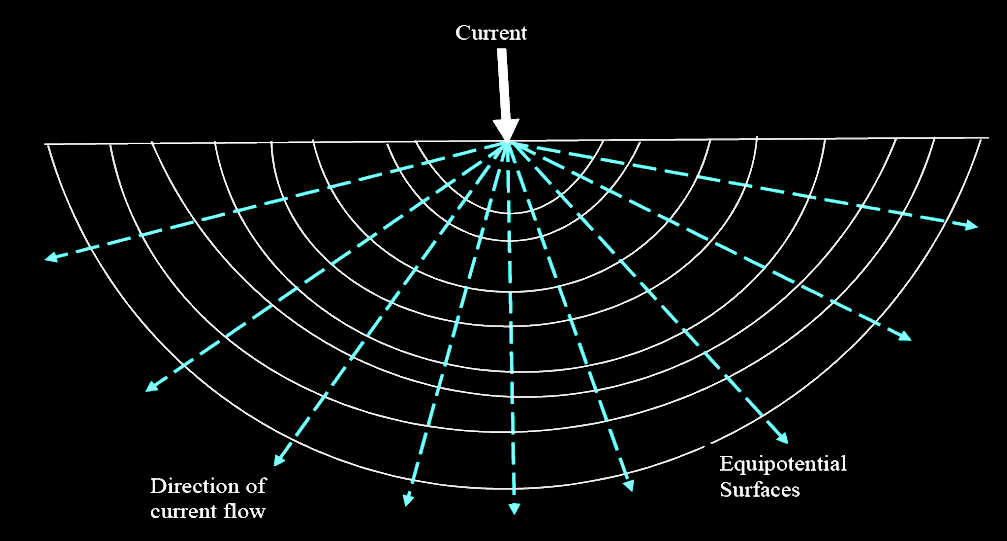
\includegraphics[width=0.7\linewidth]{Figures/Resistivity/OneElectrodeHomoHalfspace_Aizebeokhai_SResanEss2010.png}
 
     \tiny[Aizebeokhai et al., 2010]
   \end{center}
   %\end{PointSix}
 \end{frame}


 \begin{frame}
  \begin{PointSix}{Current flow through the sub-surface}
    \small
    Consider a homogeneous conducting halfspace, with constant resistivity $\rho$, under an insulating medium. Let there be a point electrode at the surface
injecting a steady current I. The current flows to a distributed \alert{sink nearby}. Find the electrostatic potential, the electric field, and consequently the pattern of current flow in the sub-surface.

    [cf. Telford Chapter 8, online resources resistivity 1 and resistivity 2.]
  \end{PointSix}
\end{frame}


\begin{frame}
  \begin{PointSix}{Current flow through the sub-surface}
   % RESISTOR with battery and arrow
   \begin{center}
    \begin{tikzpicture}
      \coordinate (A) at (8,0);
      \coordinate (C) at (3,-3);
      \draw [thick] (0,0.0) -- (8,0.0);
      \draw [->, line width = 1mm] (2,0.5) -- (2,-0.5) node[xshift=1.0cm,yshift=1.0cm,midway,left] {\small current $\vec{I}$};
      \draw [<-, line width = 1mm] (6,0.5) -- (6,-0.5) node[xshift=1.0cm,yshift=1.0cm,midway,left] {\small current $\vec{I}$};
      \draw [-,dashed, line width = 0.5mm] (6,0.0) -- (C) node[xshift=0.0cm,yshift=0.3cm,midway,sloped] {${R_2}$};
      \draw [-,dashed, line width = 0.5mm] (2,0.0) -- (C) node[xshift=0.0cm,yshift=0.3cm,midway,sloped] {${R_1}$};
      \node[yshift=0.3cm] at (A) {\small Surface};
      \node[yshift=-0.3cm] at (C) {\small $P_1$};
    \end{tikzpicture}
  \end{center}
  \end{PointSix}
\end{frame}

\begin{frame}
  \begin{PointSix}{Current flow through the sub-surface}
   % RESISTOR with battery and arrow
   \begin{center}
    \begin{tikzpicture}
      \coordinate (A) at (8,0);
      \coordinate (C) at (3,-3);
      \draw [thick] (0,0.0) -- (8,0.0);
      \draw [->, line width = 1mm] (2,0.5) -- (2,-0.5) node[xshift=1.0cm,yshift=1.0cm,midway,left] {\small current $\vec{I}$};
      \draw [<-, line width = 1mm] (6,0.5) -- (6,-0.5) node[xshift=1.0cm,yshift=1.0cm,midway,left] {\small current $\vec{I}$};
      \draw [-,dashed, line width = 0.5mm] (6,0.0) -- (C) node[xshift=0.0cm,yshift=0.3cm,midway,sloped] {${R_2}$};
      \draw [-,dashed, line width = 0.5mm] (2,0.0) -- (C) node[xshift=0.0cm,yshift=0.3cm,midway,sloped] {${R_1}$};
      \node[yshift=0.3cm] at (A) {\small Surface};
      \node[yshift=-0.3cm] at (C) {\small $P_1$};
    \end{tikzpicture}
    \small Potential at $P_1$ due to electrode at input 1
    $$
    \phi_1 = \frac{I\rho}{2\pi R_1}
    $$
  \end{center}
  \end{PointSix}
\end{frame}

\begin{frame}
  \begin{PointSix}{Current flow through the sub-surface}
   % RESISTOR with battery and arrow
   \begin{center}
    \begin{tikzpicture}
      \coordinate (A) at (8,0);
      \coordinate (C) at (3,-3);
      \draw [thick] (0,0.0) -- (8,0.0);
      \draw [->, line width = 1mm] (2,0.5) -- (2,-0.5) node[xshift=1.0cm,yshift=1.0cm,midway,left] {\small current $\vec{I}$};
      \draw [<-, line width = 1mm] (6,0.5) -- (6,-0.5) node[xshift=1.0cm,yshift=1.0cm,midway,left] {\small current $\vec{I}$};
      \draw [-,dashed, line width = 0.5mm] (6,0.0) -- (C) node[xshift=0.0cm,yshift=0.3cm,midway,sloped] {${R_2}$};
      \draw [-,dashed, line width = 0.5mm] (2,0.0) -- (C) node[xshift=0.0cm,yshift=0.3cm,midway,sloped] {${R_1}$};
      \node[yshift=0.3cm] at (A) {\small Surface};
      \node[yshift=-0.3cm] at (C) {\small $P_1$};
    \end{tikzpicture}
    \small Potential at $P_1$ due to electrode at output 2
    $$
    \phi_2 = -\frac{I\rho}{2\pi R_2}
    $$
  \end{center}
  \end{PointSix}
\end{frame}

\begin{frame}
  \begin{PointSix}{Current flow through the sub-surface}
   % RESISTOR with battery and arrow
   \begin{center}
    \begin{tikzpicture}
      \coordinate (A) at (8,0);
      \coordinate (C) at (3,-3);
      \draw [thick] (0,0.0) -- (8,0.0);
      \draw [->, line width = 1mm] (2,0.5) -- (2,-0.5) node[xshift=1.0cm,yshift=1.0cm,midway,left] {\small current $\vec{I}$};
      \draw [<-, line width = 1mm] (6,0.5) -- (6,-0.5) node[xshift=1.0cm,yshift=1.0cm,midway,left] {\small current $\vec{I}$};
      \draw [-,dashed, line width = 0.5mm] (6,0.0) -- (C) node[xshift=0.0cm,yshift=0.3cm,midway,sloped] {${R_2}$};
      \draw [-,dashed, line width = 0.5mm] (2,0.0) -- (C) node[xshift=0.0cm,yshift=0.3cm,midway,sloped] {${R_1}$};
      \node[yshift=0.3cm] at (A) {\small Surface};
      \node[yshift=-0.3cm] at (C) {\small $P_1$};
    \end{tikzpicture}
    \small Joint potential is additive superposition:
    $$
    V = \frac{I\rho}{2\pi}\left(\frac{1}{R_1} - \frac{1}{R_2} \right)
    $$
  \end{center}
  \end{PointSix}
\end{frame}

\begin{frame}
  \begin{PointSix}{Current flow through the sub-surface}
   % RESISTOR with battery and arrow
   \begin{center}
    \begin{tikzpicture}
      \coordinate (A) at (8,0);
      \coordinate (C) at (3,-3);
      \draw [thick] (0,0.0) -- (8,0.0);
      \draw [->, line width = 1mm] (2,0.5) -- (2,-0.5) node[xshift=1.0cm,yshift=1.0cm,midway,left] {\small current $\vec{I}$};
      \draw [<-, line width = 1mm] (6,0.5) -- (6,-0.5) node[xshift=1.0cm,yshift=1.0cm,midway,left] {\small current $\vec{I}$};
      \draw [-,dashed, line width = 0.5mm] (6,0.0) -- (C) node[xshift=0.0cm,yshift=0.3cm,midway,sloped] {${R_2}$};
      \draw [-,dashed, line width = 0.5mm] (2,0.0) -- (C) node[xshift=0.0cm,yshift=0.3cm,midway,sloped] {${R_1}$};
      \node[yshift=0.3cm] at (A) {\small Surface};
      \node[yshift=-0.3cm] at (C) {\small $P_1$};
    \end{tikzpicture}
    \small \alert{Visualize equipotential lines to anticipate current flow.}
    % $$
    % \phi = \frac{I\rho}{2\pi}\left(\frac{1}{R_1} - \frac{1}{R_2} \right)
    % $$
  \end{center}
  \end{PointSix}
\end{frame}

\begin{frame}{Current flow through the sub-surface}
     \begin{center}
      \begin{PointSix}{Current flow through the sub-surface}
          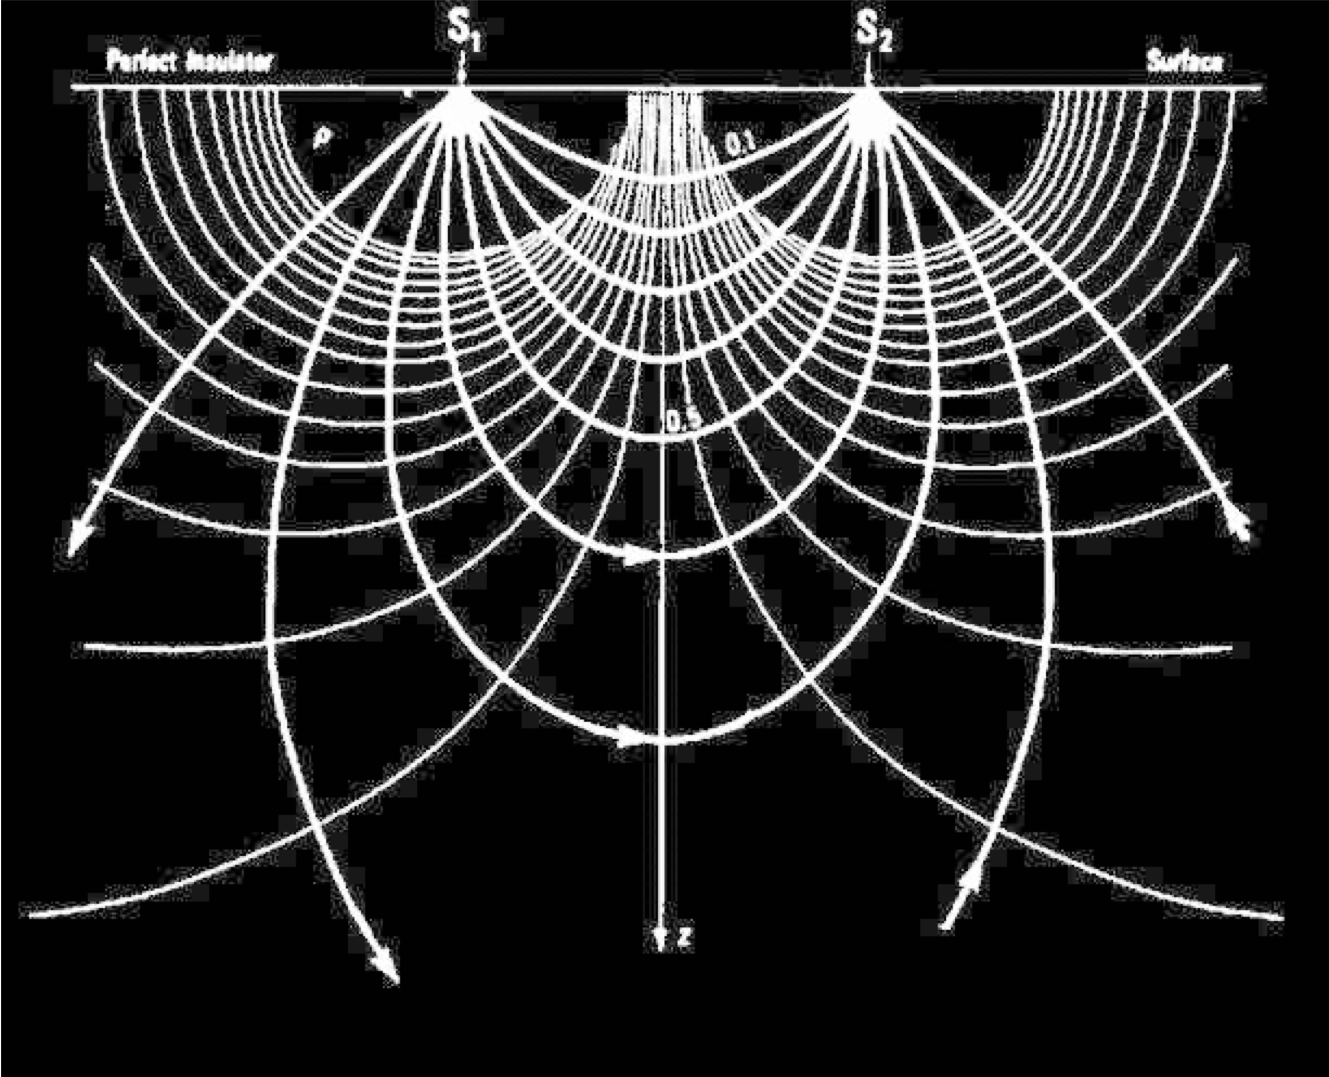
\includegraphics[width=0.7\linewidth]{Figures/Resistivity/TwoElectrodeHomoHalfspace.png}
    \end{PointSix}
   \end{center}
 \end{frame}



\begin{frame}
  \begin{PointSix}{Current flow through the sub-surface}
   \small Measuring the potential drop $V$ and the injected current $I$ is in principle enough to determine the (yet spatially homogeneous) resistivity in the sub-surface. However, in practice four electrodes are needed. Why?
   \alert{At the current electrodes there is a contact resistance depending on how the electrode is coupled to the ground. As the current is significant at this location, so is the contact resistance (Ohm's law). This will inhibit repeatability and falsify results if the potential drop is measured at this location as well.}
  \end{PointSix}
\end{frame}


\begin{frame}
  \begin{PointSix}{Principle of the resistivity method}
   % RESISTOR with battery and arrow

    \begin{tikzpicture}
      
      \newcommand\EMF{\mathcal{E}};
      \colorlet{Icol}{blue!50!black}
      \colorlet{Ccol}{orange!90!black}
      \colorlet{Rcol}{Karminrot}
      \colorlet{loopcol}{red!90!black!25}
      \colorlet{pluscol}{red!60!black}
      \colorlet{minuscol}{blue!60!black}
      \tikzstyle{EMF}=[battery1,l=$\EMF$];
      \tikzstyle{internal R}=[R,color=Rcol,Rcol,l=$r$,/tikz/circuitikz/bipoles/length=30pt];
      \tikzstyle{loop}=[->,red!90!black!25];
      \tikzstyle{loop label}=[loopcol,fill=white,scale=0.8,inner sep=1];
      \tikzstyle{thick R}=[R,color=Rcol,thick,Rcol,l=$R$];
      
      \begin{scope}[rotate=-90,transform shape]
        \fill[pattern = crosshatch dots,pattern color = brown!80!red] (0.5,-0.5) rectangle ++(6,9);
        \node[rotate=90] at (0.25,1.5) {Surface};
        \draw (0,7) to [short,*-] (0.,7) 
        to[R,color=Rcol,thick,l={{{{\rotatebox[origin=c]{90}{$R_{c2}$}}}}}] (4,7) 
        to[R,color=Rcol,thick,l={{{{\rotatebox[origin=c]{90}{$R$}}}}}] (4,0) 
        to[R,color=Rcol,thick,l={{{{\rotatebox[origin=c]{90}{$R_{c1}$}}}}}] (0,0) 
        to [short,-*] (0,0);
        \node[rotate=90,above] at (0,7) {$+$};
        \node[rotate=90,above] at (0,0) {$-$};
        \node[rotate=90] at (0,4) {$\Delta V$};
          %  \draw[->,red] (0.5, 2.15) --++ (1.2,0) node[midway,above=1] {current $I$};
          %  \draw[->,red] (0.5,-0.15) --++ (1.2,0) node[midway,below=1] {electron flow};
          \end{scope}
    \end{tikzpicture}
  \end{PointSix}
\end{frame}


\begin{frame}
  \begin{PointSix}{Current flow through the sub-surface}
   \small Solution to overcome the contact resistance: Measure the potential drop with two different electrodes at a different location and without injecting a current (i.e. the contact resistance is then unimportant.)
  \end{PointSix}
\end{frame}

\begin{frame}
  \begin{PointSix}{Principle of the resistivity method}
   % RESISTOR with battery and arrow

    \begin{tikzpicture}
      
      \newcommand\EMF{\mathcal{E}};
      \colorlet{Icol}{blue!50!black}
      \colorlet{Ccol}{orange!90!black}
      \colorlet{Rcol}{Karminrot}
      \colorlet{loopcol}{red!90!black!25}
      \colorlet{pluscol}{red!60!black}
      \colorlet{minuscol}{blue!60!black}
      \tikzstyle{EMF}=[battery1,l=$\EMF$];
      \tikzstyle{internal R}=[R,color=Rcol,Rcol,l=$r$,/tikz/circuitikz/bipoles/length=30pt];
      \tikzstyle{loop}=[->,red!90!black!25];
      \tikzstyle{loop label}=[loopcol,fill=white,scale=0.8,inner sep=1];
      \tikzstyle{thick R}=[R,color=Rcol,thick,Rcol,l=$R$];
      
      \begin{scope}[rotate=-90,transform shape]
        \fill[pattern = crosshatch dots,pattern color = brown!80!red] (0.5,-0.5) rectangle ++(6,9);
       % \node[rotate=90] at (0.25,1.5) {Surface};
        \draw (0,7)
        to[R,color=Rcol,thick,l={{{{\rotatebox[origin=c]{90}{$R_{c2}$}}}}}] (4,7) 
        to[R,color=Rcol,thick,l={{{{\rotatebox[origin=c]{90}{$R$}}}}}] (4,0) 
        to[R,color=Rcol,thick,l={{{{\rotatebox[origin=c]{90}{$R_{c1}$}}}}}] (0,0) 
        to [ammeter, color=white] (0,7);
        \node[rotate=90,above] at (0,7) {$+$};
        \node[rotate=90,above] at (0,0) {$-$};
       % \node[rotate=90] at (0,4) {$\Delta V$};
          %  \draw[->,red] (0.5, 2.15) --++ (1.2,0) node[midway,above=1] {current $I$};
          %  \draw[->,red] (0.5,-0.15) --++ (1.2,0) node[midway,below=1] {electron flow};
        \end{scope}
        \draw[-,color=white] (2,-0.8) -- (2,1.2);
        \draw[-,color=white] (2,1.2) -- node[above] {$\Delta$ U} (5,1.2);
        \draw[-,color=white] (5,1.2) -- (5,-0.8);
    \end{tikzpicture}
  \end{PointSix}
\end{frame}

\begin{frame}
  \begin{PointSix}{Terminology (A, M, N, B)}
   % RESISTOR with battery and arrow

    \begin{tikzpicture}
      
      \newcommand\EMF{\mathcal{E}};
      \colorlet{Icol}{blue!50!black}
      \colorlet{Ccol}{orange!90!black}
      \colorlet{Rcol}{Karminrot}
      \colorlet{loopcol}{red!90!black!25}
      \colorlet{pluscol}{red!60!black}
      \colorlet{minuscol}{blue!60!black}
      \tikzstyle{EMF}=[battery1,l=$\EMF$];
      \tikzstyle{internal R}=[R,color=Rcol,Rcol,l=$r$,/tikz/circuitikz/bipoles/length=30pt];
      \tikzstyle{loop}=[->,red!90!black!25];
      \tikzstyle{loop label}=[loopcol,fill=white,scale=0.8,inner sep=1];
      \tikzstyle{thick R}=[R,color=Rcol,thick,Rcol,l=$R$];
      
      \begin{scope}[rotate=-90,transform shape]
        \fill[pattern = crosshatch dots,pattern color = brown!80!red] (0.5,-0.5) rectangle ++(6,9);
       % \node[rotate=90] at (0.25,1.5) {Surface};
        \draw (0,7)
        to[R,color=Rcol,thick,l={{{{\rotatebox[origin=c]{90}{$R_{c2}$}}}}}] (4,7) 
        to[R,color=Rcol,thick,l={{{{\rotatebox[origin=c]{90}{$R$}}}}}] (4,0) 
        to[R,color=Rcol,thick,l={{{{\rotatebox[origin=c]{90}{$R_{c1}$}}}}}] (0,0) 
        to [ammeter, color=white] (0,7);
        \node[rotate=90,above] at (0,7) {$B$};
        \node[rotate=90,above] at (0,0) {$A$};
   
       % \node[rotate=90] at (0,4) {$\Delta V$};
          %  \draw[->,red] (0.5, 2.15) --++ (1.2,0) node[midway,above=1] {current $I$};
          %  \draw[->,red] (0.5,-0.15) --++ (1.2,0) node[midway,below=1] {electron flow};
        \end{scope}
        \draw[-,color=white] (2,-0.8) -- (2,1.2);
        \draw[-,color=white] (2,1.2) -- node[above] {$\Delta$ U} (5,1.2);
        \draw[-,color=white] (5,1.2) -- (5,-0.8);
        \draw[<->,color=green,line width=0.75mm] (2,-0.8) -- (0.0,-0.8) node[midway,below] {$r_1$};
        \draw[<->,color=green,line width=0.75mm] (2.0,-0.8) -- (7.0,-0.8) node[midway,below] {$r_2$};
        \draw[<->,color=green,line width=0.75mm] (0.0,-1.5) -- (5.0,-1.5) node[midway,below] {$r_3$};
        \draw[<->,color=green,line width=0.75mm] (5.0,-1.5) -- (7.0,-1.5) node[midway,below] {$r_4$};
        \node[above] at (2,1.2) {$M$};
        \node[above] at (5,1.2) {$N$};
    \end{tikzpicture}
  \end{PointSix}
\end{frame}

\begin{frame}
  \begin{PointSix}{Current flow through the sub-surface}
   \small Solution to overcome the contact resistance at electrodes A, B: Measure the potential drop with two different electrodes (M,N) at a different location and without injecting a current (i.e. the contact resistance is then unimportant.
   \\
   \vspace{1cm}
   \small \alert{What is the potential drop \textit{at the surface} measured between M and N?}
  \end{PointSix}
\end{frame}


\begin{frame}
  \begin{PointSix}{Current flow through the sub-surface}
   Four electrode setup:
   $$
    \Delta V = \frac{I\rho}{2\pi}\left((\frac{1}{r_1}- \frac{1}{r_2})-(\frac{1}{r_3}-\frac{1}{r_4})\right)
   $$
  \end{PointSix}
\end{frame}

\begin{frame}
  \begin{PointSix}{Current flow through the sub-surface}
   \small Four electrode setup:
   $$
    \Delta V = \frac{I\rho}{2\pi}\left((\frac{1}{r_1}- \frac{1}{r_2})-(\frac{1}{r_3}-\frac{1}{r_4})\right)
   $$
   $$
   \rho = \frac{ \Delta V}{I}\underbrace{2\pi\left((\frac{1}{r_1}- \frac{1}{r_2})-(\frac{1}{r_3}-\frac{1}{r_4})\right)^{-1}}_{\text{Konfiguration factor} K}
  $$
  $$
    \boxed{\rho = \frac{2\pi \Delta V}{I} K}
  $$
  \end{PointSix}
\end{frame}
\begin{frame}
  \begin{PointSix}{Apparant vs true resistivity}
   \small In an ideal case with homogenous sub-surface properties the resistivity does not depend on the specific measurement setup. In practice, however, due to lateral and vertical inhomogeneities the resistivity will change with changing electrode setup (also because the intercepted current flow follows a different path). We call:
    $$
    \boxed{\rho_a = \frac{2\pi \Delta V}{I} K}
    $$
  the \alert{apparant resistivity} which is to a certain degree diagnostic but does not correspond directly to the \textit{true resistivity}, which can only be obtain through inversion. 
  \end{PointSix}
\end{frame}

\begin{frame}{Array Types}
  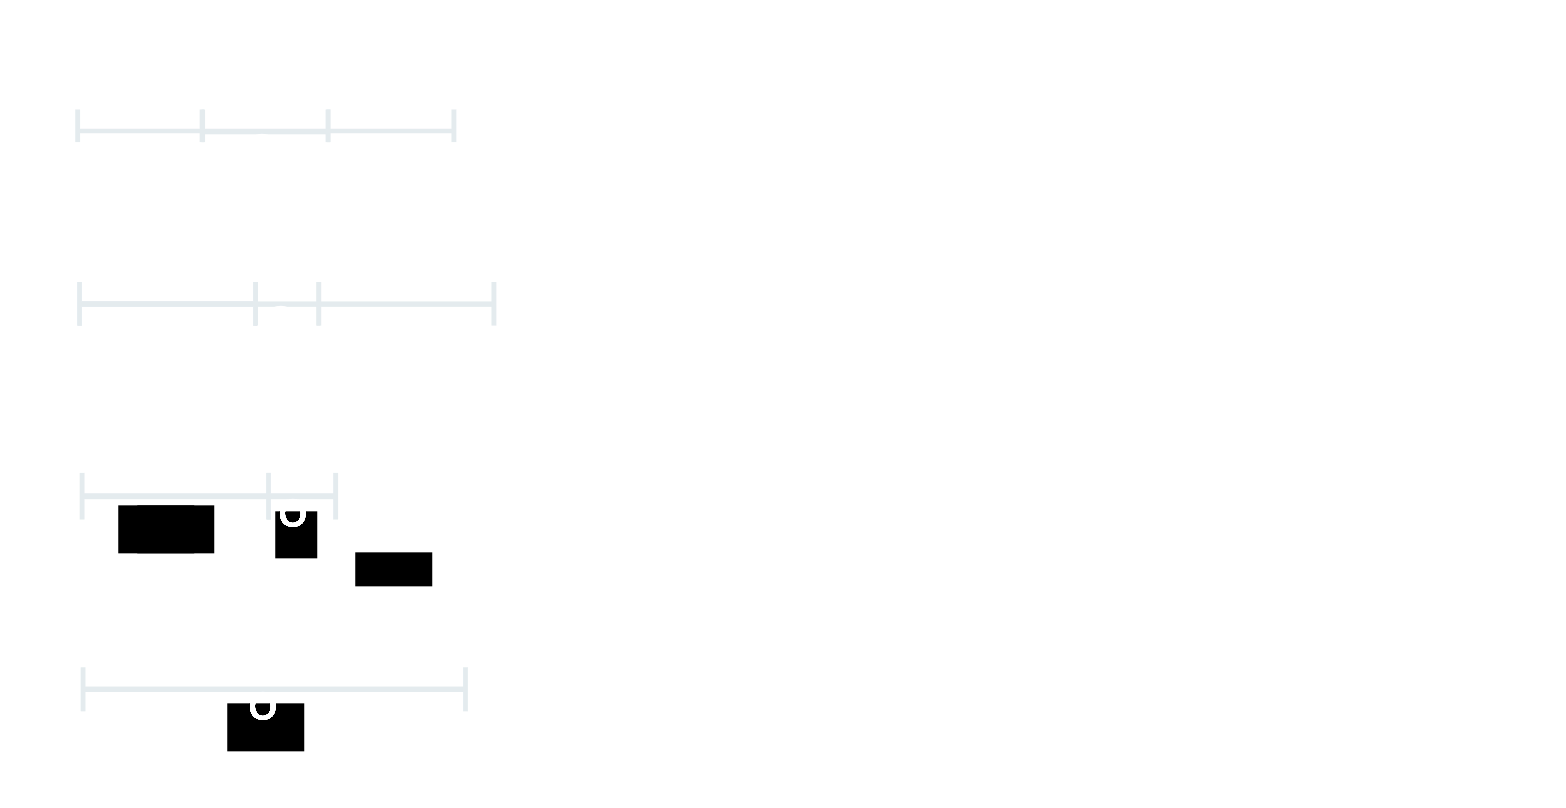
\includegraphics[width=0.9\linewidth]{Figures/Resistivity/ArrayTypes.png}
\end{frame}

\begin{frame}{Array Types}
  % http://www.ukm.edu.my/rahim/Resistivity%20lecture.htm
  \begin{PointSix}
    Applied Array types depend on:
    \begin{itemize}
      \item feasibility in the field in terms of cable lengths and movement of electrodes
      \item sensitivity to lateral (Schlumberger) and vertical (Wenner)
    \end{itemize}
  \end{PointSix}
\end{frame}


\begin{frame}{Current flow through the sub-surface with multiple layers}
  \begin{center}
    %\begin{PointSix}{Current flow through the sub-surface}
        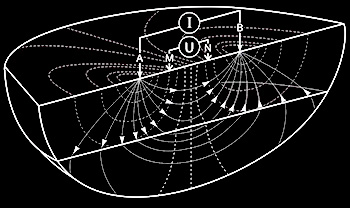
\includegraphics[width=0.5\linewidth]{Figures/Resistivity/SchlumbergerSounding_BGR.jpg}

        \tiny [BGR, Hannover]

        \small Electrical currents are refracted at boundaries with differing resistivities (conservation of charges for the normal component).
    %\end{PointSix}

\end{center}
\end{frame}

\begin{frame}{Current flow through the sub-surface with multiple layers}
  \begin{center}
    %\begin{PointSix}{Current flow through the sub-surface}
        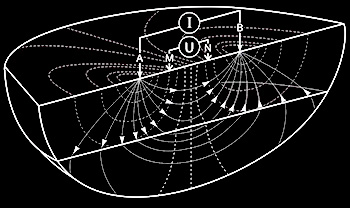
\includegraphics[width=0.5\linewidth]{Figures/Resistivity/SchlumbergerSounding_BGR.jpg}

        \tiny [BGR, Hannover]

        \small In general: The further apart the electrode spacing, the deeper the signal penetration.
    %\end{PointSix}

\end{center}
\end{frame}

\begin{frame}{Principal of vertical sounding}
  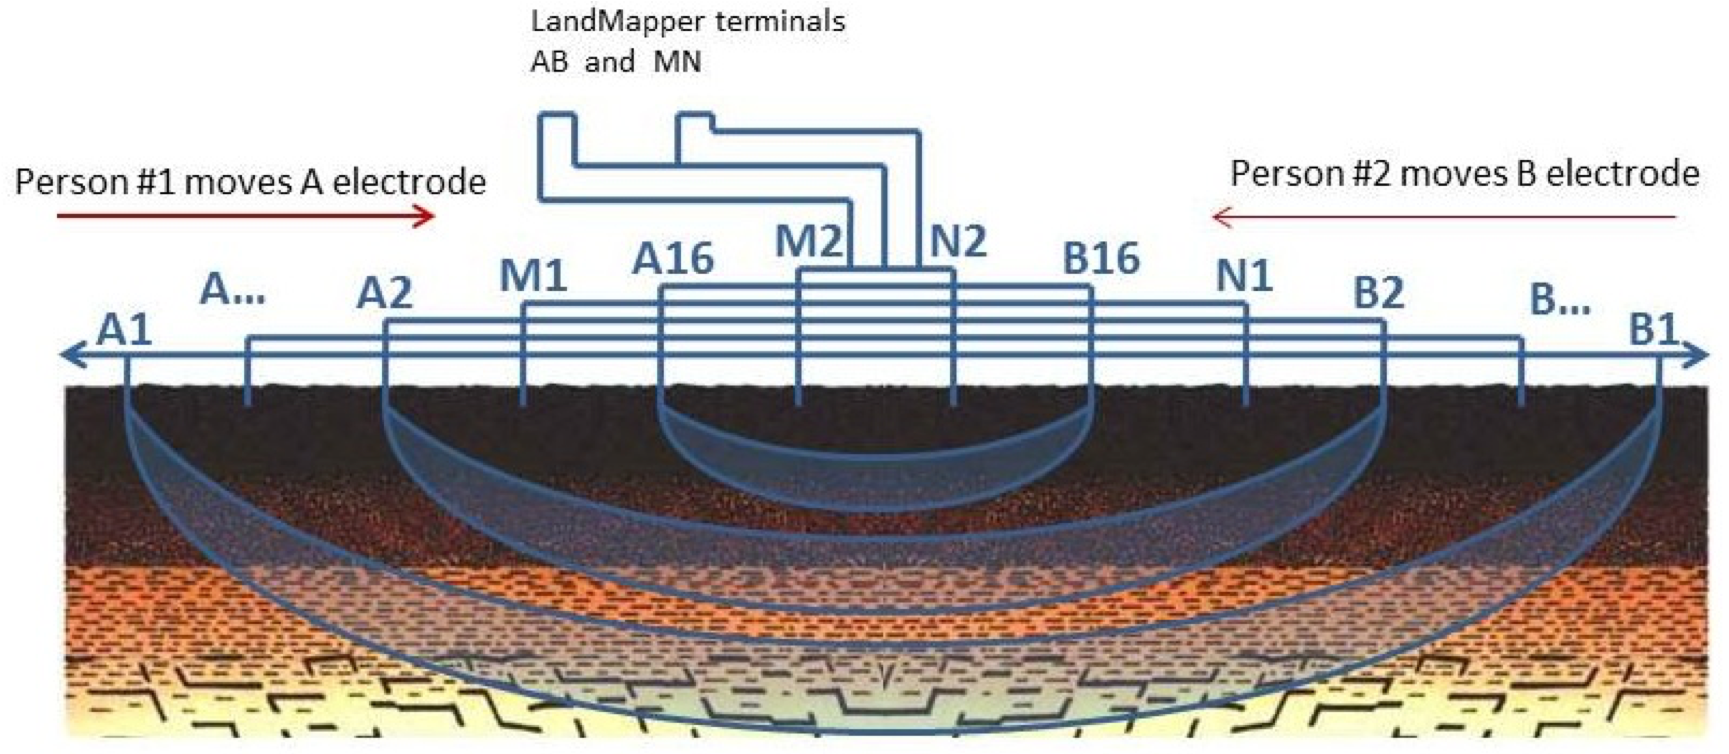
\includegraphics[width=0.9\linewidth]{Figures/Resistivity/VerticalSounding_GeoscienceEG.png}
   \small \alert{Discuss some firsts order interpretation of vertical sounding curves (AB/2 log vs $\rho_a$ log) in class}
\end{frame}

\begin{frame}
  \begin{PointSix}{Principal of vertical sounding}
    \small
    \begin{itemize}
      \item Shallowest and deepest part of sounding curve can rapidly be estimated, but interpretation of intermediate layering is more difficult.
      \item The inverse problem remains ambiguous and requires good a-priori knowledge for informed guessing.
      \item Forward modelling is helpful in the interpretation (example with PyGimli) even without applying rigours inverse theory.
  \end{itemize}
\end{PointSix}
\end{frame}

\begin{frame}
  \begin{PointSix}{Learning Goals}
    \begin{itemize}
      \item \alert{Understand the principle of the resistivity method.}
      \item \alert{Understand basic electrostatic principles.}
      \item \alert{Understand principles of vertical sounding.}
    \end{itemize}
  \end{PointSix}
\end{frame}